\chapter{Architektura aplikace}
\hspace{14pt} Tato kapitola pojednává o tom, jak je aplikace sestavená. Věnuje se konfiguračnímu nastavení, prezentační vrstvě, vrstvě aplikační logiky a struktuře databáze. Jsou zde zmíněny klíčové prvky aplikace.
\section{Konfigurační nastavení aplikace}
\hspace{14pt} Gradle je buildovací nástroj používaný v Android vývoji k automatizaci procesu sestavení aplikace. Umožňuje spravovat závislosti, optimalizovat kód a zajišťovat kompatibilitu mezi různými verzemi Androidu. Gradle používá soubory s příponou .gradle.kts k definování konfigurace projektu. V mé aplikaci se nacházejí následující Gradle soubory. \textbf{build.gradle (Project-level)} se nachází v kořenové složce projektu a obsahuje globální konfigurace pro celý projekt. Definuje správu pluginů a repozitářů, odkud se stahují závislosti. \textbf{build.gradle (Module-level)} se nachází v modulu DayPlanner. Pokud by bylo modulů více, každý by měl svůj vlastní Gradle soubor. Zde jsou definována specifická nastavení aplikace, jako je verze SDK, závislosti a optimalizace. \textbf{settings.gradle} určuje, jaké moduly jsou součástí projektu, a definuje správu závislostí a repozitářů pro celý projekt. Tyto soubory dohromady řídí způsob, jakým se aplikace sestavuje.

\newpage

Zde jsou uvedeny důležité závislosti mého projektu. \textbf{Firebase BoM} používá se k automatickému správnému verzování závislostí souvisejících s Firebase. Díky tomu není nutné u každého Firebase produktu uvádět konkrétní verzi. \textbf{Firebase Analytics} poskytuje analytická data o používání aplikace, jako je chování uživatelů a interakce s aplikací.\textbf{ Firebase Realtime Database} je cloudová databáze umožňující synchronizaci dat v reálném čase mezi zařízeními. \textbf{Firebase Authentication} slouží k autentizaci uživatelů v aplikaci, například pomocí e-mailu, hesla nebo přihlášení přes Google. \textbf{Google Play Services Auth} poskytuje funkce pro autentizaci uživatele přes Google účet. MPAndroidChart je knihovna pro vykreslování grafů a vizualizaci dat v aplikaci.
\begin{lstlisting}[style=javastyle,caption = {build.gradle},label = {lst:build.gradle}]
dependencies {
    implementation(platform("com.google.firebase:firebase-bom:33.8.0"))
    implementation("com.google.firebase:firebase-analytics")
    implementation("com.google.firebase:firebase-database")
    implementation("com.google.firebase:firebase-auth:23.1.0")
    implementation("com.google.android.gms:play-services-auth:21.3.0")
    implementation("com.github.bumptech.glide:glide:4.16.0")
    implementation("com.github.PhilJay:MPAndroidChart:v3.1.0")
}
\end{lstlisting}

V adresáři DayPlanner/app je soubor google-services.json, který obsahuje všechna důležitá data a konfigurace, aby se uživatel mohl úspěšně přihlásit přes Google účet.

\newpage
\section{Adresářová struktura}
\hspace{14pt} Nyní bude krátce zmíněno, jak je aplikace rozdělená do adresářů. V adresáři java/com.example.dayplanner se nachází backend aplikace a v adresáři res/ se nachází frontend aplikace. Jelikož bylo v backendu poměrně veliké množství tříd, rozhodl jsem třídy rozčlenit do jednotlivých balíčků(package) pojmenovaných podle funkcionality. 

\dirtree{%
.1 DayPlanner/.
  .2 app/.
    .3 src/.
      .4 main/.
        .5 java/.
            .6 com.example.dayplanner/.
                .7 auth/.
                .7 main/.
                .7 notifications/.
                .7 settings/.
                .7 statistics.
        .5 res/.
         .6 drawable/.
         .6 layout/.
         .6 values/.
         .6 .....
}

Package auth se stará o autentikaci uživatele. Uživatel se může přihlásit přes Google nebo přes vlastní email. V případě, že si uživatel zakládá účet přes email, přijde mu na email odkaz na ověření. Jedině pokud uživatel email ověří, tak může pokračovat dále do aplikace a založit si účet. Package main se člení dál. Nachází se v něm funkcionalita pro časovou osu, vybírání dne z kalendáře, modely pro jednorázové a opakované akce a třída main. Package notifications se stará o vytváření a posílání notifikací. V package settings se nachází logika pro ukládání nastavení uživatele a package statistics se stará o počítání statistik a vytváření přehledného UI.

Jak již bylo řečeno adresář res/ se stará o design aplikace. V podadresáři drawable se nachází xml soubory, které se pak používají v layout. Jedná se například o různé ikony, obrázky, pozadí nebo tvary. V podadresáři layout se nachází xml design pro aktivity a fragmenty. Aktivita se zpravidla skládá z více menších oddělitelných částí neboli z fragmentů. To slouží k znovupoužitelnosti a přehlednosti kódu. Pro lepší ilustraci aktivity a fragmentů je dáno k dispozici schéma níže. 

\newpage
\begin{figure}[h]
    \centering
    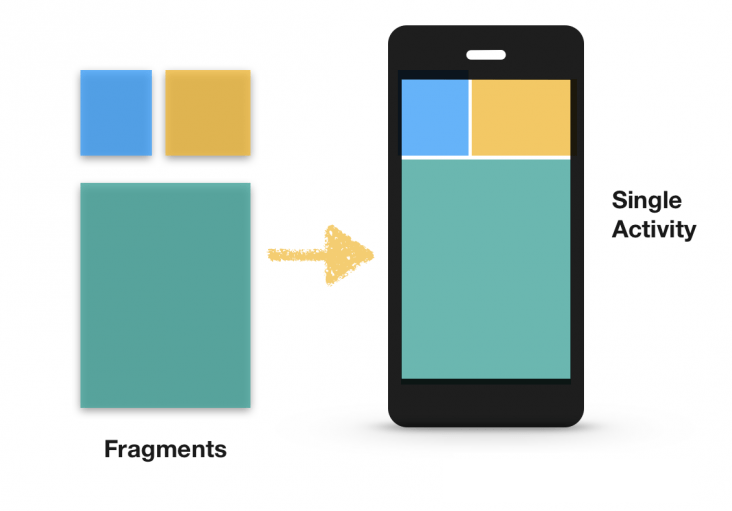
\includegraphics[width=0.7\textwidth]{images/activityfragment.png} % Adjust width as needed
    \caption{Activity \& Fragments schema}
    \label{fig:sunset} % Reference label if needed
    \vspace{0.5em} % Space between caption and source
    {\footnotesize Zdroj: https://medium.com/ibtech/activity-vs-fragment-703c749c1bbd \par} % Image source
\end{figure}

V adresáři values se nachází hodnoty. Nachází se zde hodnoty textových řetězců, polí, barev a podobně. Je zde uložen design například pro světlý a tmavý režim.

\newpage

\section{Prezentační vrstva (Frontend)}
\hspace{14pt} Tato kapitola se věnuje aktivitám, fragmentům a důležitým designovým prvkům aplikace. 

\subsection{Main activity}
\hspace{14pt} Třída main activity se skládá z několika komponent. Důležité jsou dva fragmenty. Za prvé WeeklyHeaderFragment, který je zodpovědný za ukazování dnů po týdnech, aktuální měsíc a rok a možnost vybrat si konkrétní den pomocí kalendáře. Za druhé TimelineFragment, který ukazuje časovou osu s jednorázovými a opakovanými akcemi. 
\begin{figure}[H]
    \centering
    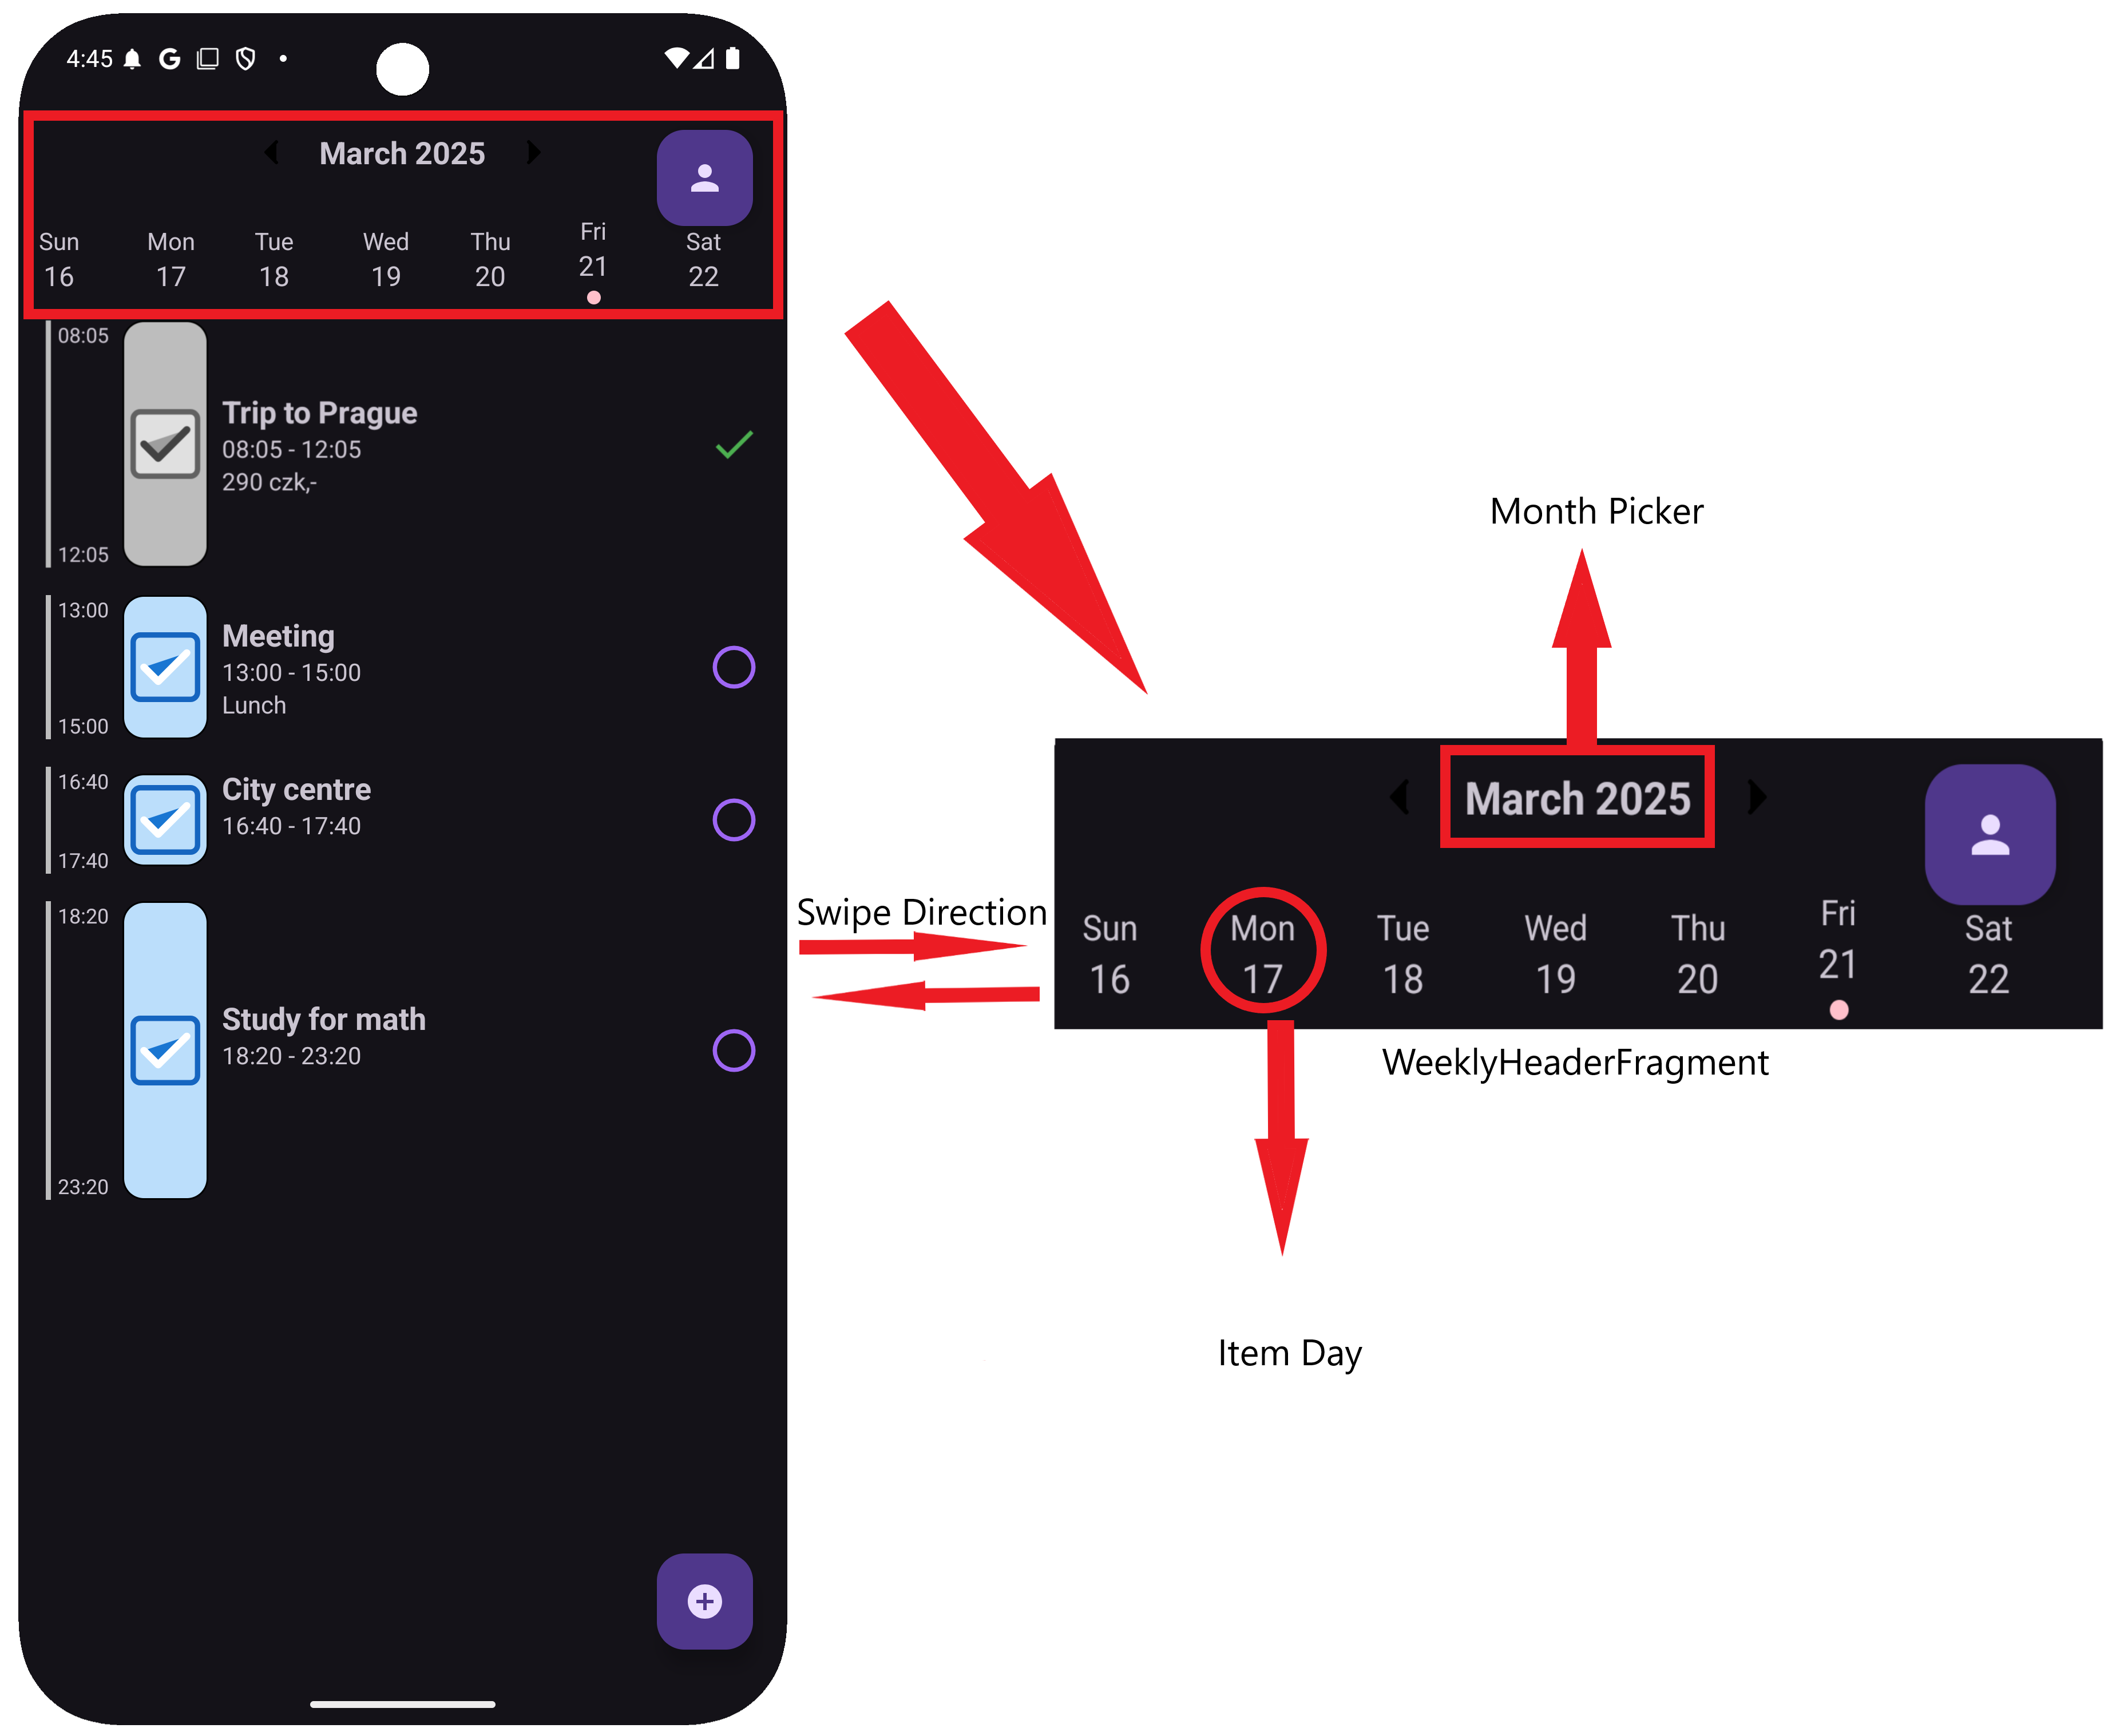
\includegraphics[width=0.9\linewidth]{images/WeeklyHeaderFragmentDetail.png}
    \caption{WeeklyHeaderFragment}
    \label{fig:enter-label}
\end{figure}

WeeklyHeaderFragment se stará o ukazování aktuálního týdne po dnech. Umožňuje uživateli pohybovat se mezi dny. Uživatel může táhnutím prstu(Swipe Direction \autoref{fig:enter-label}) posouvat týdny dopředu nebo dozadu. Pokud uživatel nechce swipovat po týdnech, může kliknout na Month Picker(\autoref{fig:enter-label}) a vybrat z kalendáře konkrétní den. Když uživatel klikne na Item Day(\autoref{fig:enter-label}), vybere tím konkrétní den a je poslán signál pomocí interface do timeLineFragment. Tento fragment získá z databáze potřebná data a zobrazí je v časové ose.

TimelineFragment získá potřebná data z databáze, seřadí jednotlivé položky podle času a upraví jejich výšku podle doby trvání. Následně je postupně pod sebou zobrazí. Jak lze vidět, jednorázové akce se dají pomocí tlačítka(circle sign) označit za dokončené. Poté změní barvu na černobílou a zobrazí se u nich fajfka indikující(finished task, tick sign), že je úkol hotový. U opakovaných akcí může uživatel pohybovat seekbar, aby zadal hodnotu. Pokud je návyk například sníst denně 3000 kalorií, stává se seekbar poněkud nešikovný a nepřesný, protože počítá hodnotu podle toho, jak daleko uživatel potáhl prstem. Proto si pomocí tlačítka "+"(add progress button) může hodnotu zadat manuálně. Může buď celou hodnotu nastavit znovu nebo ke stávající hodnotě přidat pokrok.

\begin{figure}[H]
    \centering
    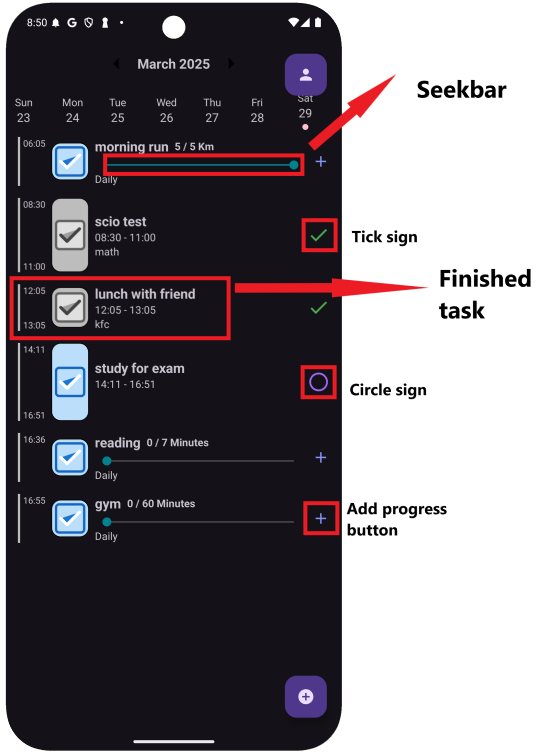
\includegraphics[width=0.6\linewidth]{images/timeline.png}
    \caption{Timeline Fragment}
    \label{fig:enter-label}
\end{figure}


\newpage

\subsection{Statistiky}
\hspace{14pt} Statistiky v aplikaci mají za cíl co nejintuitivněji a nejpřehledněji zobrazit uživateli jeho pokrok, aby snadno zjistil, kde má prostor pro zlepšení, a zároveň se mohl radovat z dosažených úspěchů. Na základě vlastních zkušeností považuji za velmi užitečné na konci každého měsíce vyhodnotit plnění návyků, a proto jsou statistiky vždy rozděleny podle jednotlivých měsíců. Uživatel si mezi nimi může snadno přepínat pomocí nástroje Month Picker(\autoref{fig:Statistics}).  

Nejdůležitější součástí statistik je ukazatel celkové úspěšnosti v daném měsíci, který se zobrazuje v sekci Overall Month Progress(\autoref{fig:Statistics}). Tento ukazatel může zobrazovat průměrnou úspěšnost všech sledovaných návyků dohromady nebo jednoho konkrétního, který si uživatel vybere ze seznamu. Výpočet celkové úspěšnosti vychází z průměru všech dní v měsíci. Pokud například jeden den splní návyky jen na padesát procent a druhý den na sto procent, celková úspěšnost bude sedmdesát pět procent. Kolem procentuálního ukazatele se nachází barevný kruh, který vizuálně odráží úspěšnost v daném měsíci. Barevné spektrum přechází od červené, která značí nízkou úspěšnost, přes oranžovou a žlutou až po zelenou, která indikuje vysokou úspěšnost. Pokud uživatel za daný měsíc nezaznamenal žádné údaje, kruh zůstává šedý.  

Pod tímto ukazatelem se nachází kalendářová mapa, která rozděluje měsíc na jednotlivé dny. Každý den je zobrazen samostatně a jeho úspěšnost je vyjádřena pomocí kruhového indikátoru. Díky tomu má uživatel detailní přehled o tom, jak se mu v průběhu měsíce dařilo.  

Kromě vizualizace jednotlivých dní aplikace zobrazuje i dvě další klíčové statistiky. První z nich je počet perfektních dní, tedy takových dní, kdy uživatel splnil všechny své návyky na sto procent. Druhou důležitou statistikou je nejdelší nepřerušená sekvence perfektních dní, označovaná jako "streak". Tato hodnota ukazuje, jak dlouhou dobu se uživateli dařilo udržet si pravidelný návykový režim bez přerušení.  

Pokud si uživatel zobrazí statistiky pro konkrétní návyk, získá ještě jednu doplňkovou informaci. V takovém případě se mu zobrazí také celkový počet splnění návyku za daný měsíc. Tato hodnota může být vyjádřena v různých jednotkách, například v minutách strávených cvičením, v celkové vzdálenosti v kilometrech nebo ve spálených kaloriích.  
\newpage
Pokud aplikace zaznamená, že v průběhu měsíce došlo ke změně cílové hodnoty návyku, zobrazí se uživateli interaktivní graf. Tento graf umožňuje sledovat, jak se cílová hodnota měnila v průběhu měsíce, a pomáhá lépe pochopit, jak se uživatelův výkon a cíle vyvíjely.  

Celkově jsou statistiky navrženy tak, aby uživateli poskytly nejen detailní přehled o jeho pokroku, ale také ho motivovaly k dalšímu zlepšování a pomohly mu lépe pochopit jeho vlastní návyky.
\begin{figure}[H]
    \centering
    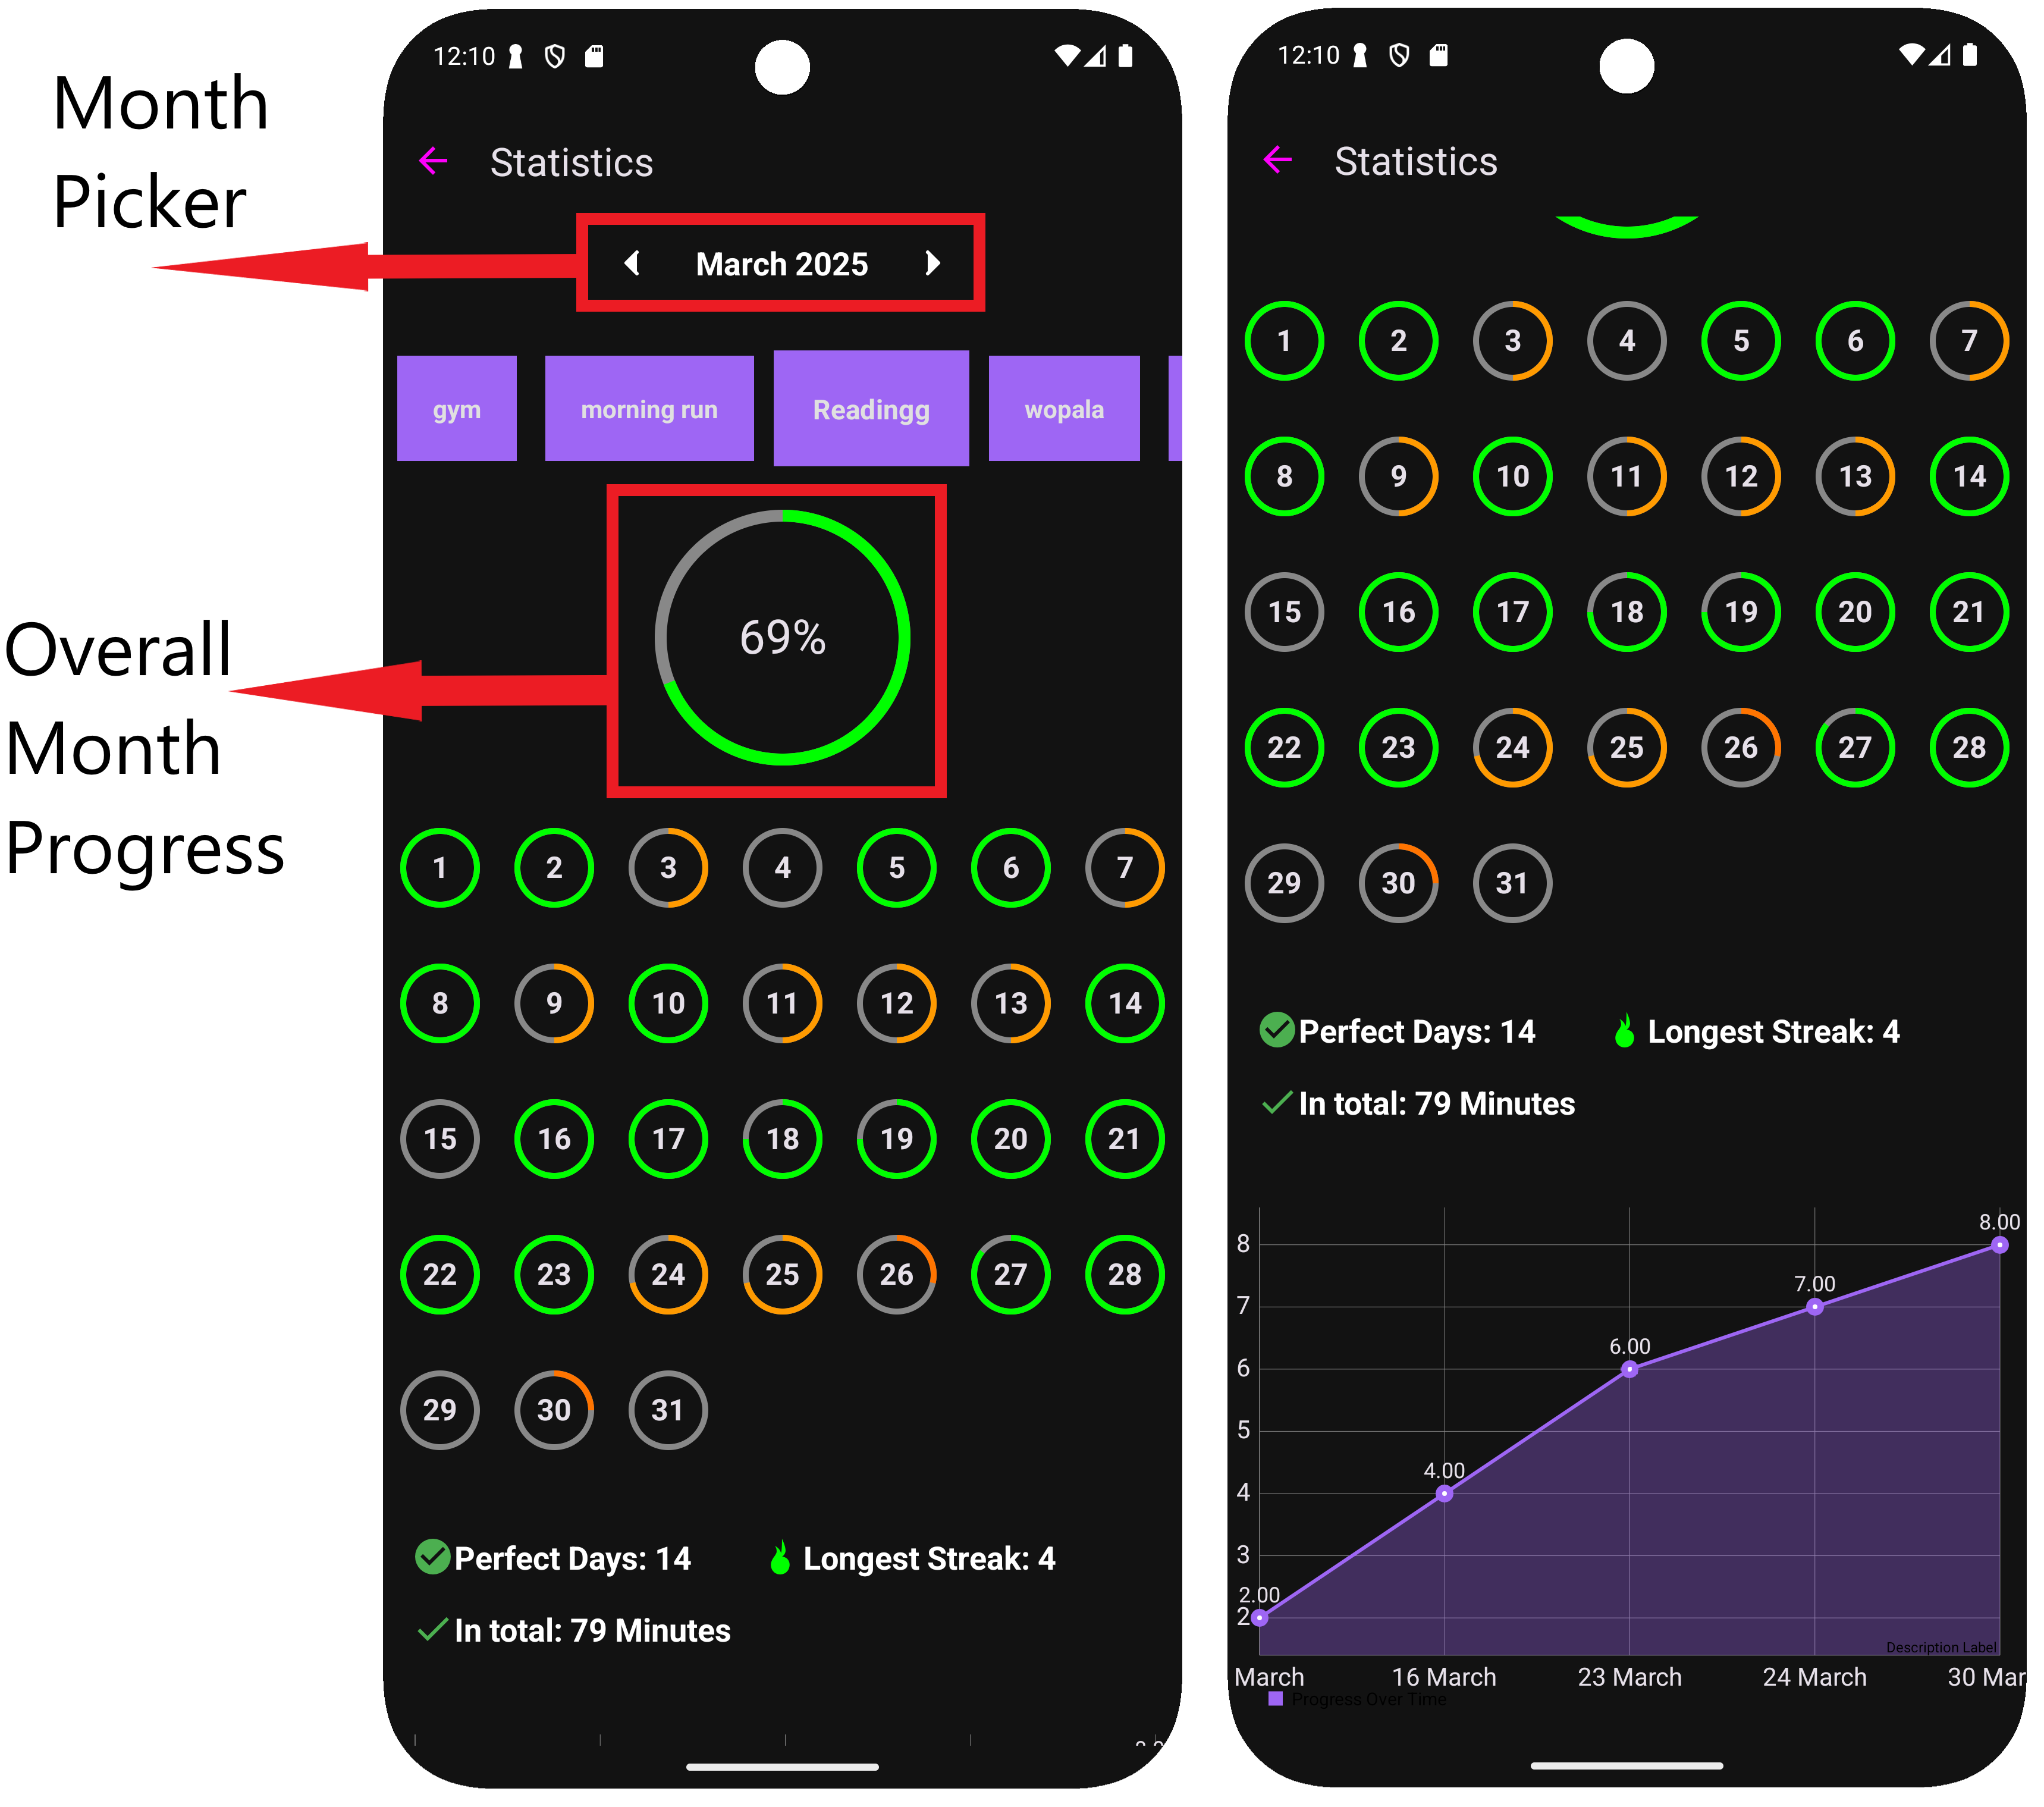
\includegraphics[width=1\linewidth]{images/supercuper.png}
    \caption{Statistics}
    \label{fig:Statistics}
\end{figure}

\newpage

\subsection{Tmavý a světlý režim}
\hspace{14pt} Tato aplikace podporuje světlý a tmavý režim pomocí Material 3 a SQLite databáze pro uchování preferencí uživatele. Hodnoty motivů jsou definovány ve values/themes.xml a values-night/themes.xml. ThemePreferenceHelper.java se stará o ukládání uživatelem preferovaného motivu do lokálního úložiště a pochopitelně zajišťuje i získání této hodnoty, aby s ní aplikace mohla pracovat. 

Konkrétněji to vypadá následovně. Barvy pro motivy jsou definované stejně, jediné co se liší jsou hodnoty barev(\autoref{lst:SvMotiv}, \autoref{lst:TmMotiv}).

\begin{lstlisting}[style=xmlstyle,caption = {Hodnoty světlého motivu},label = {lst:SvMotiv}]
<style name="Base.Theme.DayPlanner" parent="Theme.Material3.DayNight.NoActionBar">
    <item name="colorPrimary">@color/lavender</item>
    <item name="colorOnPrimary">@color/colorOnPrimaryLight</item>
    <item name="colorPrimaryVariant">@color/lavender</item>
    <item name="colorSecondary">@color/colorSecondaryLight</item>
    ...
</style>
\end{lstlisting}

\begin{lstlisting}[style=xmlstyle,caption = {Hodnoty tmavého motivu},label = {lst:TmMotiv}]
<style name="Base.Theme.DayPlanner" parent="Theme.Material3.DayNight.NoActionBar">
    <item name="colorPrimary">@color/darkGrey</item>
    <item name="colorOnPrimary">@color/black</item>
    <item name="colorPrimaryVariant">@color/darkGrey</item>
    <item name="colorSecondary">@color/colorSecondaryDark</item>
    ...
</style>
\end{lstlisting}
\newpage
Hodnoty barev, na které odkazuje `themes.xml`, se nacházejí v `colors.xml`(\autoref{lst:HodnotyMotivu}). 
\begin{lstlisting}[style=xmlstyle,caption = {Hodnoty barev},label = {lst:HodnotyMotivu}]
<color name="colorPrimaryLight">#CE9932</color>
<color name="colorPrimaryDark">#2F0385</color>
\end{lstlisting}

O správné nastavování motivu a ukládání preference do databáze se stará již zmíněná třída ThemePreferencesHelper.java. Hlavní metody jsou setThemePreference(\autoref{lst:setThemePreference}), která uloží motiv do lokální databáze, aby se uživateli po každém opětovném zapnutí zobrazoval jím zvolený motiv.

\begin{lstlisting}[style=javastyle,caption = {setThemePreference},label = {lst:setThemePreference}]
public void setThemePreference(String theme) {
    SQLiteDatabase db = this.getWritableDatabase();
    db.execSQL("UPDATE preferences SET theme = ? WHERE id = 1", new String[]{theme});
    db.close();
}
\end{lstlisting}

Když se aplikace inicializuje, tedy uživatel ji zapne, je potřeba hodnotu z databáze získat. K tomu slouží metoda getThemePreference(\autoref{lst:getThemePreference}). Když hodnotu získám, pak mohu během inicializace aplikace ve třídě main nastavit barevné hodnoty podle uživatelem preferovaného motivu. Při startu aplikace se načte uložená preference a aplikuje se odpovídající motiv(\autoref{lst:nastaveníMotivu}).

\begin{lstlisting}[style=javastyle,caption = {getThemePreference},label = {lst:getThemePreference}]
public String getThemePreference() {
    SQLiteDatabase db = this.getReadableDatabase();
    String theme = "light"; // Default Value
    Cursor cursor = db.rawQuery("SELECT theme FROM preferences WHERE id = 1", null);
    if (cursor.moveToFirst()) {
        theme = cursor.getString(0);
    }
    cursor.close();
    db.close();
    return theme;
}
\end{lstlisting}
\begin{lstlisting}[style=javastyle,caption = {Nastavení motivu},label = {lst:nastaveníMotivu}]
ThemePreferencesHelper dbHelper = new ThemePreferencesHelper(this);
if (dbHelper.getThemePreference().equals("dark")) {
    AppCompatDelegate.setDefaultNightMode(AppCompatDelegate.MODE_NIGHT_YES);
} else {
    AppCompatDelegate.setDefaultNightMode(AppCompatDelegate.MODE_NIGHT_NO);
}
\end{lstlisting}

Pokud uživatel změní režim v nastavení aplikace, preference se uloží a téma se přepne pomocí metod v themePreferenceHelper.
\begin{lstlisting}[style=javastyle,caption = {Změnění motivu},label = {lst:nastaveníMotivu}]
switchMode.setOnClickListener(new View.OnClickListener() {
@Override
public void onClick(View v) {
    if (nightMode) {
        AppCompatDelegate.setDefaultNightMode(AppCompatDelegate.MODE_NIGHT_NO);
        themePreferencesHelper.setThemePreference("light");
    } else {
        AppCompatDelegate.setDefaultNightMode(AppCompatDelegate.MODE_NIGHT_YES);
        themePreferencesHelper.setThemePreference("dark");
    }
    nightMode = !nightMode;
}
});
\end{lstlisting}

Tento přístup dynamicky nastavuje hodnoty barev pro různé komponenty aplikace podle toho, co si uživatel vybral za motiv. Motiv se navíc ukládá do lokálního úložiště, takže kdykoliv se uživatel do aplikace vrátí, zobrazí se mu aplikace ve správném motivu.
\newpage
\section{Vrstva aplikační logiky (Backend)}
\hspace{14pt} Tato kapitola pojednává o klíčových funkcích, algoritmech a strukturách, které se v mé práci nacházejí.
\subsection{Rozdělení logiky}
\hspace{14pt} Moje aplikace často využívá těchto tří komponent: Activity, Fragment a RecyclerView. Každá z těchto součástí má svůj specifický účel a společně tvoří strukturovaný a efektivní způsob práce s uživatelským rozhraním.  

Activity je základní stavební jednotka aplikace, která představuje jednu obrazovku. Každá aplikace obsahuje alespoň jednu aktivitu, která je prvním vstupním bodem pro uživatele. Aktivita řídí celý proces zobrazení, reaguje na uživatelské akce a může obsahovat další komponenty, jako jsou fragmenty nebo seznamy dat.  

Fragment je menší část uživatelského rozhraní, která může být vložena do aktivity. Hlavní výhodou fragmentů je jejich flexibilita – umožňují dynamické změny v rozhraní bez nutnosti přepínání celých aktivit. Fragmenty lze kombinovat na jedné obrazovce (viz. kapitola frontend) a znovu použít v různých částech aplikace. Aktivita obvykle spravuje více fragmentů a mezi nimi přepíná podle potřeby.  

RecyclerView je způsob, jak efektivně zobrazovat seznamy nebo mřížky dat. Používá adaptér, který propojuje data s jednotlivými položkami seznamu, a ViewHolder, který optimalizuje vykreslování tím, že znovu používá již vytvořené pohledy.  

Typickým příkladem propojení těchto komponent je aplikace, kde hlavní aktivita obsahuje více fragmentů s přehledem dat, a tyto fragmenty využívají RecyclerView's pro zobrazení seznamu položek.  

\newpage

\subsection{Autentizace a přihlášení uživatele}
\hspace{14pt} Uživatel se může přihlásit dvěma způsoby. Buď pomocí emailu a nebo může pokračovat přes Google účet. Authentication activity(\autoref{fig:AuthActivtiy}) je hlavní třída zajišťující přihlášení uživatele. 
\\ 
\begin{figure}[H]
    \centering
    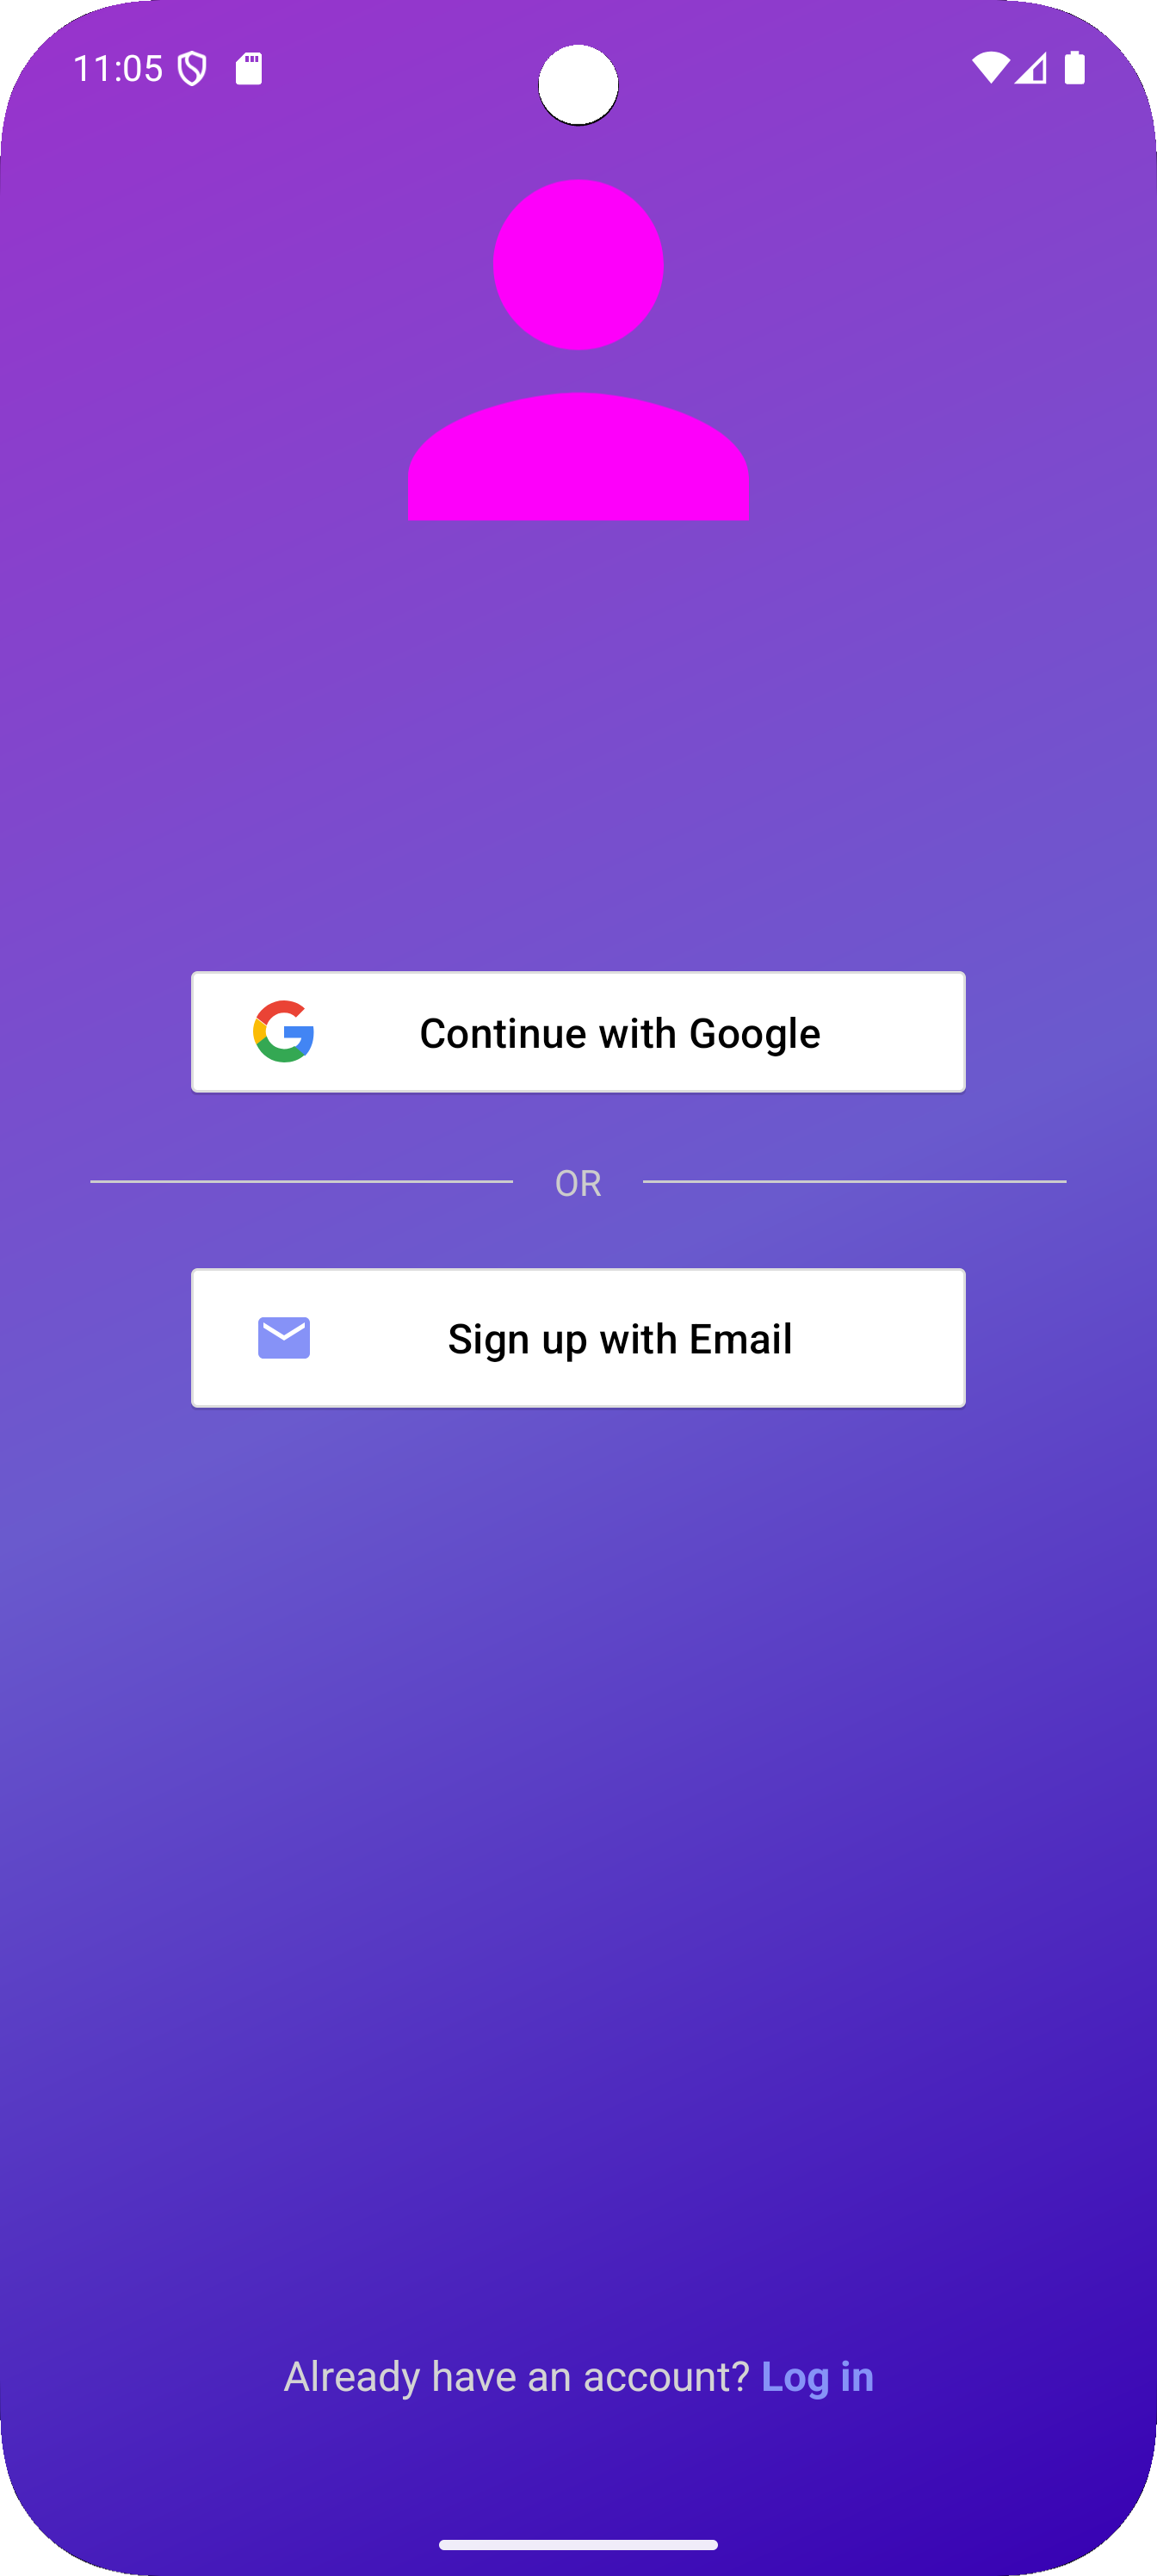
\includegraphics[width=0.4\linewidth]{images/auth.png}
    \caption{Authentication Activity}
    \label{fig:AuthActivtiy}
\end{figure}
Níže je adresářová struktura balíčku auth.
\\
\dirtree{%
.1 auth/.
    .2 google/.
        .3 GoogleLoginFragment.java.
    .2 login/.
        .3 EmailLoginActivity.java.
    .2 signin/.
        .3 EmailSignInActivity.java.
    .2 AuthenticationActivity.java.
}

\newpage

Google přihlášení v aplikaci je implementováno ve třídě GoogleLoginFragment. Tento fragment se pak používá v authentication activity jako tlačítko, které má veškerou potřebnou funkcionalitu.  Přihlášení probíhá přes Firebase Authentication a Google Sign-In API. Fragment inicializuje GoogleSignInClient (\autoref{lst:googleSignInOptions}) s odpovídajícími možnostmi (GoogleSignInOptions), kde je vyžadován ID token a e-mail. Po kliknutí na tlačítko pro přihlášení se spustí přihlašovací intent přes activityResultLauncher (\autoref{lst:signInIntent}), který zachytí výsledek přihlášení. Pokud je přihlášení úspěšné, získá se účet Google a předá se metodě firebaseAuthWithGoogle(). Ta pomocí GoogleAuthProvider vytvoří přihlašovací pověření a provede autentizaci ve Firebase (\autoref{lst:GoogleAuthProvider}). Při úspěchu se zobrazí potvrzení a aplikace přesměruje uživatele do hlavní aktivity.

\begin{lstlisting}[style=javastyle,caption = {googleSignInOptions},label = {lst:googleSignInOptions}]
GoogleSignInOptions googleSignInOptions = new GoogleSignInOptions.Builder(GoogleSignInOptions.DEFAULT_SIGN_IN)
    .requestIdToken(getString(R.string.client_id))
    .requestEmail()
    .build();
googleSignInClient = GoogleSignIn.getClient(
    requireContext(), googleSignInOptions);
\end{lstlisting}        

\begin{lstlisting}[style=javastyle,caption = {signInIntent},label = {lst:signInIntent}]
Intent signInIntent = googleSignInClient.getSignInIntent();
activityResultLauncher.launch(signInIntent);
\end{lstlisting}          

\begin{lstlisting}[style=javastyle,caption = {GoogleAuthProvider},label = {lst:GoogleAuthProvider}]
AuthCredential credential = GoogleAuthProvider.getCredential(account.getIdToken(), null);
firebaseAuth.signInWithCredential(credential).addOnCompleteListener(task -> {
    if (task.isSuccessful()) {
        startActivity(new Intent(getActivity(), MainActivity.class));
        requireActivity().finish();
    }
});
\end{lstlisting} 

\newpage

Uživatel se může zaregistrovat nebo přihlásit pomocí svého emailu. EmailSignIn activity  slouží k registraci nových uživatelů a EmailLoginActivity  umožňuje přihlášení existujících uživatelů. Pro registraci uživatel zadává svůj email a heslo. Heslo je pro bezpečnost zadáváno dvakrát, obě hesla se musí shodovat a pole nesmí být prázdná.

\begin{lstlisting}[style=javastyle,caption = {Create New User},label = {lst:CreateNewUser}]
firebaseAuth.createUserWithEmailAndPassword(email, password).addOnCompleteListener(new OnCompleteListener<AuthResult>() {
    @Override
    public void onComplete(@NonNull Task<AuthResult> task) {
        progressDialog.hide();
        if (task.isSuccessful()) {
            handleEmailVerification(firebaseAuth, 
                "User registered successfully, Please verify your email address", 
                "Something went wrong");
        } else {
            Toast.makeText(EmailSignInActivity.this, "Something went wrong", Toast.LENGTH_SHORT).show();
            Log.d("USR", "EXCEPTION: " + task.getException().toString());
        }
        Intent intent = new Intent(EmailSignInActivity.this, EmailLoginActivity.class);
        startActivity(intent);
    }
});
\end{lstlisting} 

Firebase metoda createUserWithEmailAndPassword(\autoref{lst:CreateNewUser}) provede registraci. Pokud je registrace úspěšná, je uživatel přesměrován pomocí intent na EmailLoginActivity a zároveň je mu na emailovou adresu poslán odkaz pro ověření emailu. Pokud uživatel email neověří kliknutím na odkaz, nemůže se do aplikace přihlásit.

\begin{lstlisting}[style=javastyle,caption = {handleEmailVerification},label = {lst:handleEmailVerification}]
public void handleEmailVerification(FirebaseAuth firebaseAuth, String message_on_successful, String message_on_not_successful) {
    if (firebaseAuth.getCurrentUser() != null) {
        firebaseAuth.getCurrentUser().sendEmailVerification().addOnCompleteListener(new OnCompleteListener<Void>() {
            @Override
            public void onComplete(@NonNull Task<Void> task) {
                if(task.isSuccessful()) {
                    Toast.makeText(EmailSignInActivity.this, message_on_successful, Toast.LENGTH_SHORT).show();
                    editEmail.setText("");
                    editPassword.setText("");
                    editConfirmPassword.setText("");
                } else {
                    Toast.makeText(EmailSignInActivity.this, message_on_not_successful, Toast.LENGTH_SHORT).show();
                }
            }
        });
    }
}

\end{lstlisting}    

Funkce handleEmailVerification(\autoref{lst:handleEmailVerification}) pošle prostřednictvím firebaseAuth email uživateli a kontroluje výsledek. Pokud byl email úspěšně odeslán, zobrazí se uživateli pozitivní zpráva. V opačném případě se uživateli zobrazí zpráva o neúspěchu. Pokud vše proběhlo v pořádku, pokračuje přihlášení v EmailLoginActivity. Zde se uživatel může přihlásit. Pokud pole pro heslo a email nejsou prázdná, podívá se funkce, zda byl email ověřen pomocí isEmailVerified() a zkontroluje také, zda je heslo shodné s heslem ve Firebase. Pokud alespoň jedna podmínka neplatí, přihlášení se nezdaří. Pokud vše proběhne bez komplikací je uživatel přesměrován do MainActivity. \newpage

\begin{lstlisting}[style=javastyle,caption = {SignInWithEmailAndPassword},label = {lst:SignInWithEmailAndPassword}]
mAuth.signInWithEmailAndPassword(email, password).addOnCompleteListener(new OnCompleteListener<AuthResult>() {
    @Override
    public void onComplete(@NonNull Task<AuthResult> task) {
        progressDialog.hide();
        if(task.isSuccessful()) {
            if(mAuth.getCurrentUser().isEmailVerified()) {
                Intent intent = new Intent(EmailLoginActivity.this, MainActivity.class);
                startActivity(intent);
            } else {
                Toast.makeText(EmailLoginActivity.this, "Please verify your email address", Toast.LENGTH_SHORT).show();
            }
        } else {
            Toast.makeText(EmailLoginActivity.this, task.getException().getMessage(), Toast.LENGTH_SHORT).show();
        }
    }
});

\end{lstlisting}

Může se stát, že email nemusí přijít nebo ho uživatel například omylem smaže. Proto je v EmailLoginActivity tlačítko, které po kliknutí pošle verifikaci emailu znovu(\autoref{lst:SendEmailVerification}).

\begin{lstlisting}[style=javastyle,caption = {Send Email Verification},label = {lst:SendEmailVerification}]
sendVerificationLink.setOnClickListener(new View.OnClickListener() {
    @Override
    public void onClick(View view) {
        if (mAuth.getCurrentUser() != null) {
            sendVerificationEmail(mAuth.getCurrentUser());
        } else {
            // Handles blank fields and parsing and non existing users
            Whole code is in the actual project
        }
    }
});
\end{lstlisting}

\newpage

\subsection{Habit}
\hspace{14pt} Model návyku (Habit) je třída implementovaná v Javě, která spravuje všechny podstatné informace o individuálním návyku v aplikaci. Je navržena pro ukládání dat do Firebase Realtime Database, která umožňuje flexibilní ukládání dat.

\begin{figure}[H]
    \centering
    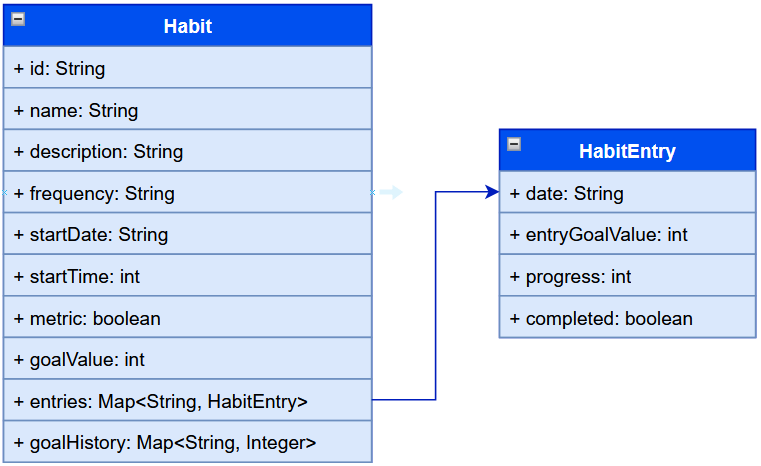
\includegraphics[width=1\linewidth]{images/HABIT.png}
    \caption{Habit Model}
    \label{fig:habit-model}
\end{figure}

Každý návyk obsahuje řadu klíčových atributů, které definují jeho charakteristiku a průběh. Patří mezi ně jedinečné identifikační číslo, název, popis, frekvence provádění, datum zahájení, čas zahájení, měřítko a cílová hodnota. Systém také uchovává dynamické informace jako aktuální sérii úspěchů (current streak) a nejdelší sérii úspěchů (longest streak).

Další součástí modelu jsou dvě mapy: `entries` a `goalHistory`. Mapa `entries` uchovává záznamy o jednotlivých dnech (`HabitEntry`), kde každý záznam reprezentuje postup a stav návyku v konkrétní den. Mapa `goalHistory` pak uchovává historii změn cílových hodnot pro různé datumy.

Klíčovou metodou je `isHabitVisibleOnDate()`, která určuje, zda má být návyk zobrazen v určitém dni. Metoda pracuje s různými frekvencemi:

\newpage
\begin{lstlisting}[style=javastyle,caption = {isHabitVisibleOnDate},label = {lst:isHabitVisibleOnDate}]
public boolean isHabitVisibleOnDate(String dateToCheck) {
// If check date is before the habit start date, return false
            if (checkDate.compareTo(start) < 0) {
                Log.d("Habit", "Habit start date is after the check date: " + dateToCheck + " > " + start.getTime());
                return false;
            }

    switch (frequency.toLowerCase()) {
        case "daily":
            return true; 
        case "weekly":
            return start.get(Calendar.DAY_OF_WEEK) == checkDate.get(Calendar.DAY_OF_WEEK);
        case "custom":
            String customPattern = frequency.substring(7);
            int dayOfWeekIndex = (checkDate.get(Calendar.DAY_OF_WEEK) + 5) % 7;
            boolean isVisibleCustom = customPattern.charAt(dayOfWeekIndex) != '-';
            return isVisibleCustom;
    }
    ......
}
\end{lstlisting}

Metoda `getGoalValueForDate()` umožňuje dynamicky zjistit cílovou hodnotu pro konkrétní datum, přičemž preferuje specifické hodnoty z `goalHistory` před výchozí hodnotou návyku.

Každý návyk má také své vlastní položky (HabitEntry), které reprezentují denní progress. Třída `HabitEntry` obsahuje datum, cílovou hodnotu pro daný den, aktuální postup a příznak dokončení. Metoda `updateProgress()` v této třídě automaticky spravuje postup a stanovuje, zda je úkol splněn.

V kontextu ukládání a správy dat spolupracuje `GoalManager` s modelem návyku. Poskytuje metody pro aktualizaci cílových hodnot, ukládání historie cílů a správu budoucích záznamů.

Celý model je navržen s ohledem na flexibilitu a dynamické sledování postupu uživatele při plnění jeho návyků.


\subsection{Task}
\hspace{14pt} Třída `Task`, umístěná v balíčku `com.example.dayplanner.main.tasks`, představuje model jednorázového úkolu v aplikaci DayPlanner. Tento model slouží k uchování a správě informací o jednotlivých úkolech, které uživatel zadává do aplikace. Každý úkol obsahuje specifické atributy, které umožňují jeho efektivní načítání, zpracování a vizualizaci v rámci časové osy.  

Struktura třídy zahrnuje identifikátor úkolu (`taskId`), název (`taskTitle`), volitelný popis (`taskDescription`), datum přiřazení (`taskDate`), čas začátku (`taskStartTime`), délku trvání (`taskLength`) a stav dokončení (`isCompleted`). Datum je uloženo ve formátu `ddMMyyyy`, což umožňuje snadné vyhledávání a třídění úkolů v databázi. Čas začátku a délka trvání jsou klíčové parametry pro správné umístění a vizuální reprezentaci úkolu na časové ose.  

Kromě základních getterů a setterů obsahuje třída také metodu `isValid()`, která ověřuje, zda jsou všechny klíčové atributy úkolu správně vyplněny. To zabraňuje ukládání nekompletních nebo chybných záznamů do databáze.  

\begin{figure}[H]
    \centering
    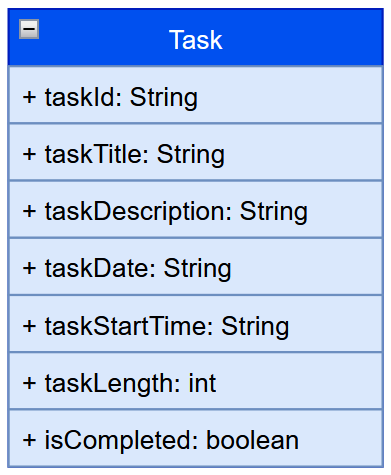
\includegraphics[width=0.4\linewidth]{images/TASK.png}
    \caption{Task Model}
    \label{fig:task-model}
\end{figure}
\newpage
\subsection{Časová osa}
\hspace{14pt} Časová osa je klíčovým prvkem aplikace DayPlanner, který uživatelům umožňuje lépe si představit svůj den a efektivně plánovat pomocí blokového plánování.

Implementace časové osy zahrnuje načítání, zpracování a vizualizaci denních aktivit. Data pocházejí ze dvou zdrojů – jednorázové úkoly jsou uloženy v lokální SQLite databázi, zatímco pravidelné návyky se spravují v cloudovém úložišti Firebase Realtime Database. Proces začíná výběrem konkrétního data, kdy TimelineFragment spouští paralelní načítání úkolů a návyků. Metoda fetchTasks() získává jednorázové úkoly z lokální databáze, zatímco fetchHabits() zpracovává data o návycích z Firebase.

Načítání návyků vyžaduje několik kroků. Základní informace, jako je název nebo datum začátku návyku, se získávají snadno. Klíčovou otázkou je ale určení aktuálního pokroku a cílové hodnoty pro vybraný den. Záznamy se vyhledávají podle data ve formátu 'ddMMyyyy' (například 15032025 pro 15. března 2025). Pokud existuje odpovídající záznam, lze z něj jednoduše získat hodnoty entryGoalValue a progress. Problém nastává, pokud záznam pro daný den neexistuje – typicky když si uživatel zobrazí návyk v konkrétní den poprvé. V takovém případě je třeba záznam vytvořit. Hodnoty date, completed a progress se nastaví na výchozí hodnoty, ale pro entryGoalValue je nutné zjistit, jaká cílová hodnota platila v daném období. K tomu slouží atribut GoalsHistory, který umožňuje určit správnou hodnotu na základě časového intervalu.

Důležitou součástí procesu je také ověření, zda by měl být návyk v daný den vůbec zobrazen. To řeší metoda isHabitVisible(), která kontroluje začátek platnosti návyku a jeho frekvenci. Například pokud návyk začal 10. března 2025 a opakuje se týdně v pondělí, nemůže být zobrazen 8. března (protože tehdy ještě neexistoval) ani 14. března (protože ten den neodpovídá nastavené frekvenci).

Po načtení všech dat se položky seřadí podle času začátku pomocí Collections.sort. Vizualizace probíhá pomocí vlastního dynamického TimelineLayoutManageru, který přizpůsobuje délku a umístění prvků podle časového rozvržení. Tento přístup umožňuje intuitivní a přehledné zobrazení aktivit, kde delší úkoly zaujímají větší prostor.

Celková architektura systému je navržena s důrazem na flexibilitu a snadnou uživatelskou interakci. Výsledkem je dynamická časová osa, která efektivně podporuje time management a poskytuje přehledný vizuální plán dne.

\newpage

\subsection{Statistiky}
\hspace{14pt} Klíčovou funkcí aplikace DayPlanner jsou již zmíněné statistiky. Zde jsou shrnuty algoritmy a výpočty použité k vytvoření smysluplných a pro uživatele zajímavých statistik.


\dirtree{%
.1 statistics/.
  .2 CustomCircularPorgressBar.java.
  .2 DailyProgress.java.
  .2 HabitListAdapter.java.
  .2 HabitProgressEntry.java.
  .2 MonthlyProgressAdapter.java.
  .2 StatisticsActivity.java.
}

Třída StatisticsActivity zpracovává a analyzuje data týkající se sledování návyků. Jádrem implementace jsou algoritmy schopné transformovat surová data o denních aktivitách do vypovídajících statistických ukazatelů.

Aplikace musí nejprve získat data z databáze, následně s nimi provést několik výpočtů a nakonec je zobrazit v prezentační vrstvě. Problém je, že dat je poměrně hodně, obzvlášť když uživatel aplikaci již nějakou dobu používá a má více návyků. Proto jsem se rozhodl data cachovat. Vždy když uživatel klikne na další měsíc, musí se počítat statistiky pro všechny viditelné návyky v daný měsíc. Proto se funkce xy prvně podívá, zda nejsou nějaká data v mezipaměti. Pokud ano zavolám funkci, která cachnuté data poskytne frontendu. V opačném případě pomocí reference na návyky získám data z Firebase a zavolám metodu processHabitData, která se postará o všechny výpočty a posílání dat do frontendu.

\begin{lstlisting}[style=javastyle,caption = {Data Cache},label = {lst:isHabitVisibleOnDate}]
private void fetchAllHabitData(String monthId) {
    if (monthDataCache.containsKey(monthId)) {
        updateUIWithCachedData(monthDataCache.get(monthId));
        return;
    }

    habitsRef.addListenerForSingleValueEvent(new ValueEventListener() {
        @Override
        public void onDataChange(DataSnapshot dataSnapshot) {
            executor.execute(() -> {
                processHabitData(dataSnapshot, monthId);
            });
        }
    });
\end{lstlisting}

Pokud uživatel klikne na konkrétní návyk, nechci ukazovat data pro všechny návyky ale jen pro jeden specifický v daném měsíci. O to se stará metoda processHabitForMonth. Jelikož jsou výpočty pro získání statistik pro jeden návyk a celý měsíc podobné, využívají stejných menších funkcí. Tím nevzniká redundantní kód a vše je přehlednější a udržitelnější. Níže jsou popsány již zmíněné menší funkce.

Algoritmus pro výpočet nejdelšího sledu (streaku) představuje klíčový prvek hodnocení konzistence uživatelova chování. Implementovaná metoda `countLongestStreak` provádí lineární průchod přes všechny denní záznamy a sleduje nepřerušenou sérii úspěšně splněných dnů. Algoritmu stačí lineárně projít pole. Vždy, když potká další hodnotu true, zvýší si počítadlo o jedna a porovná hodnotu s dosavadním maximem(dosud nejdelší nalezená posloupnost) a do proměnné dosavadního maxima uloží maximum z těchto hodnot. Perfektní dny se počítají jednoduše tak, že se nehledá nejdelší sekvence, nýbrž se jen navyšuje počítadlo o jedna vždy, když jsou všechny návyky během dne splněny na sto procent.

Graf pokroku, implementovaný pomocí knihovny MPAndroidChart, vizualizuje vývoj dat. Algoritmus `formatHabitProgressDataForChart` zajišťuje přípravu dat pro grafické zobrazení tím, že eliminuje redundantní body a zachovává pouze významné změny v hodnotách. Jednoduše řečeno hledá jen změny v cílové hodnotě návyku v průběhu měsíce a pokud takovou změnu najde, uloží si datum této změny. Pokud nejsou k dispozici dostatečná data (méně než dva body), je graf automaticky skryt, protože by byl nevypovídající.

Vizuální prezentace statistik je realizována prostřednictvím několika klíčových komponent. Lineární graf zobrazuje vývoj pokroku v čase, kruhový progress bar reprezentuje celkový měsíční pokrok a další textové prvky poskytují detailní číselné shrnutí, včetně počtu perfektních dnů a nejdelší série úspěšných dnů.
\newpage
\subsection{Notifikační systém}
\hspace{14pt} V Aplikaci sloužící k tomu, aby uživatel plnil úkoly a zlepšoval se v návycích, nesmí chybět notifikační systém neboli připomínky. To funguje následovně. Notifikace jsou naplánovány pomocí AlarmManageru, a když nastane správný čas, BroadcastReceiver je zachytí a zobrazí uživateli upozornění.

Novější verze Androidu (API 26+) vyžadují notifikační kanál. Tento kanál se vytvoří v metodě createNotificationChannel(Context context), kde se nastaví název, popis a úroveň důležitosti. Pokud kanál ještě neexistuje, systém jej vytvoří(). Bez tohoto kroku by se notifikace na novějších verzích Androidu nezobrazily.
Plánování notifikace

\begin{lstlisting}[style=javastyle,caption = {NotificationChannel},label = {lst:NotificationChannel}]

NotificationChannel channel = new NotificationChannel(CHANNEL_ID, name, importance);
channel.setDescription(description);
manager.createNotificationChannel(channel);

\end{lstlisting}

Hlavní metodou pro plánování notifikace je scheduleNotification. Tato metoda vytvoří PendingIntent, který se odešle do systému s požadavkem na spuštění v daný čas – konkrétně pět minut před začátkem úkolu().

\begin{lstlisting}[style=javastyle,caption = {alarmManager},label = {alarmManagere}]

long notificationTime = taskTimeMillis - (5 * 60 * 1000);
alarmManager.setExact(AlarmManager.RTC_WAKEUP, notificationTime, pendingIntent);

\end{lstlisting}

Před naplánováním se zkontroluje, zda aplikace má oprávnění k přesnému plánování alarmů (od API 31+), a pokud ne, uživatel je přesměrován do nastavení. Při prvním spuštění aplikace je uživatel dotázán, zda chce nebo nechce povolit notifikace. Notifikace může povolit nebo zablokovat v sekci nastavení, kdykoliv bude chtít. Jakmile systém spustí naplánovaný Broadcast, zachytí ho TaskNotificationReceiver, který zkontroluje, zda uživatel povolil notifikace v SharedPreferences.
\newpage

\begin{lstlisting}[style=javastyle,caption = {Povolení notifikací},label = {lst:notificationsEnabled}]

boolean notificationsEnabled = preferences.getBoolean("notifications_enabled", true);
if (!notificationsEnabled) return;

\end{lstlisting}


Pokud jsou notifikace povoleny, vytvoří se a zobrazí oznámení pomocí NotificationManageru().

\begin{lstlisting}[style=javastyle,caption = {Vytvoření notifikace},label = {lst:NotifikaceDesign}]

NotificationCompat.Builder builder = new NotificationCompat.Builder(context, TaskNotificationHelper.CHANNEL_ID)
        .setSmallIcon(R.drawable.ic_notification)
        .setContentTitle("Task Reminder")
        .setContentText("Your task: " + taskTitle + " starts in 5 minutes")
        .setPriority(NotificationCompat.PRIORITY_HIGH)
        .setAutoCancel(true);

\end{lstlisting}


Notifikace se zobrazí s titulem „Task Reminder“ a informací, že úkol začíná za 5 minut(\autoref{fig:task-reminder}).

\begin{figure}[H]
    \centering
    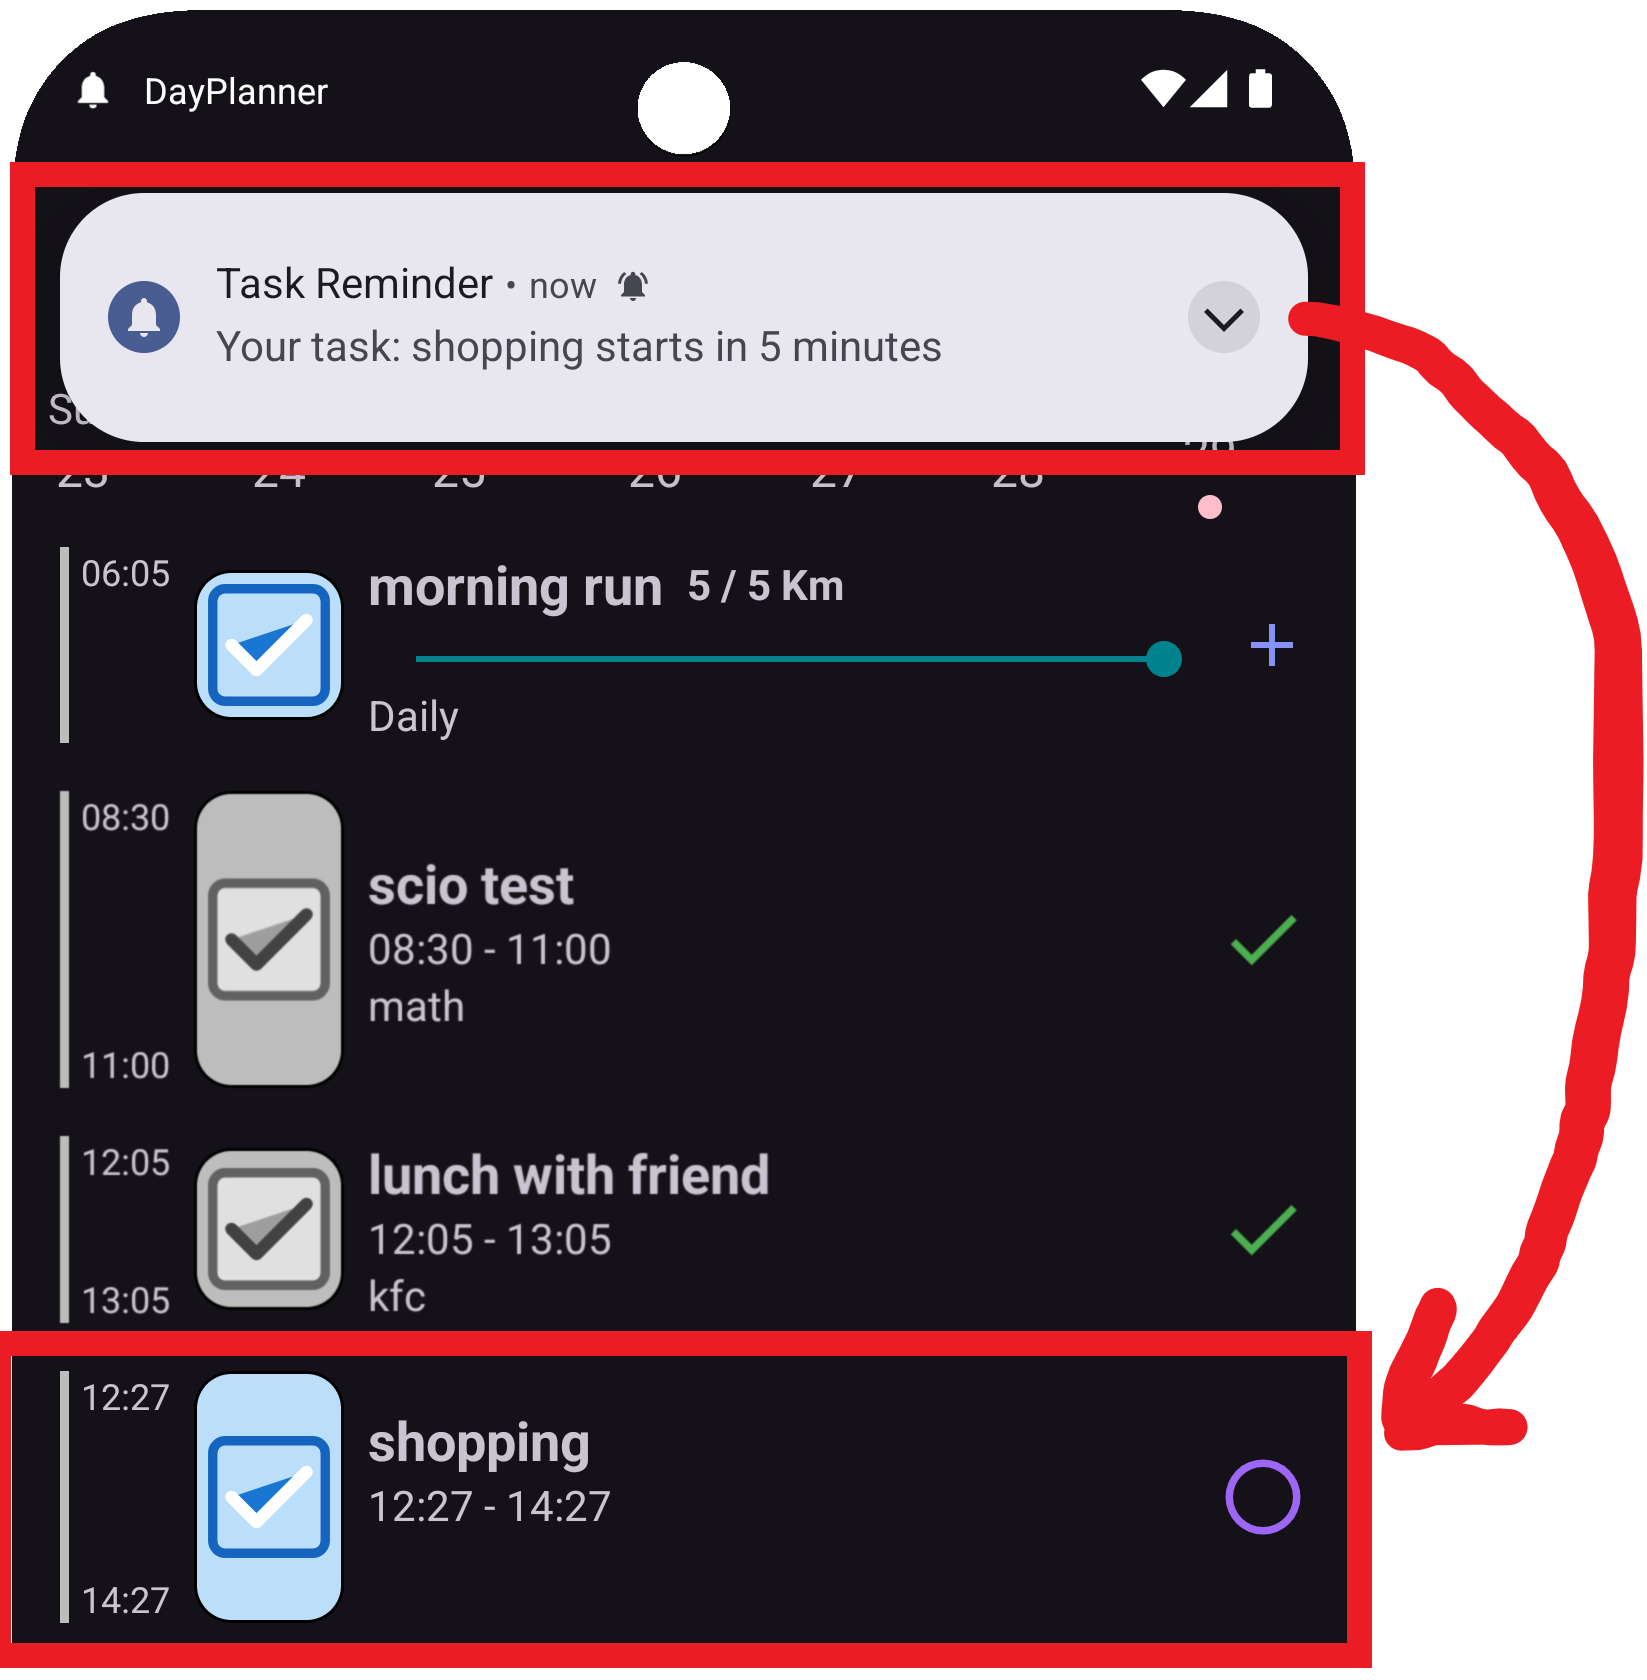
\includegraphics[width=0.5\linewidth]{images/reminderedit.png}
    \caption{Připomínka}
    \label{fig:task-reminder}
\end{figure}

\newpage

\section{Struktura databáze}
\hspace{14pt} Aplikace DayPlanner využívá kombinaci lokální databáze SQLite a cloudové databáze Firebase Realtime Database, aby zajistila optimální rovnováhu mezi offline přístupem a synchronizací dat. Lokální úložiště slouží k ukládání uživatelských preferencí, jako je nastavení tmavého režimu nebo aktivace notifikací, a také jednorázových akcí, které po splnění již nejsou pro uživatele důležité. Naopak opakované akce a návyky jsou uchovávány v cloudu, protože obsahují cenné statistiky a dlouhodobá data, o která by uživatel nechtěl přijít, například při přechodu na nové zařízení. Díky tomu jsou všechny statistiky a návyky vázány na konkrétního uživatele a jsou dostupné z jakéhokoliv telefonu. Jednorázové akce nemají takovou hodnotu z hlediska dlouhodobého sledování, a proto je jejich ukládání do Firebase nadbytečné.

Databáze pro jednorázové akce neboli tasky vypadá podobně jako samotný model Task(\autoref{fig:task-model}). Zde je schéma SQLite tabulky pro jednorázové akce(\autoref{fig:task-dbl}). 

\begin{figure}[H]
    \centering
    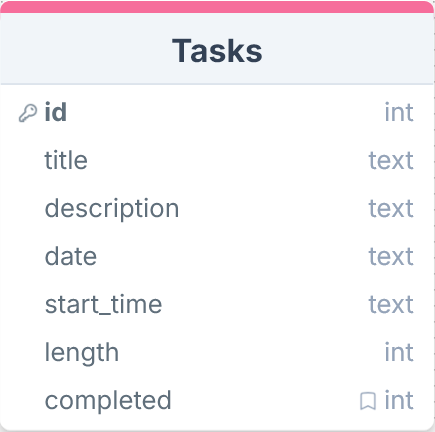
\includegraphics[width=0.5\linewidth]{images/task.png}
    \caption{SQLite Task Table}
    \label{fig:task-dbl}
\end{figure}

\newpage
\setcounter{enumiv}{4}
Firebase je takzvaná NoSQL databáze. Místo klasické relační databáze jako je například SQLite, ukládá Firebase data v takzvaných JSON objektech jako stromy. \textit{„Všechna data ve Firebase Realtime Database jsou uložena jako JSON objekty. Můžete si databázi představit jako cloudově hostovaný JSON strom. Na rozdíl od SQL databáze zde neexistují tabulky ani záznamy. Když do JSON stromu přidáte data, stanou se uzlem v existující struktuře s přiřazeným klíčem. Klíče si můžete určit sami, například pomocí uživatelských ID nebo sémantických názvů, nebo mohou být automaticky generovány pomocí metody push()"}\cite{firebase2025}. Schéma JSON stromu databáze mé aplikace je zobrazeno níže a rozděleno do dvou schémat pro lepší přehlednost. Každý uživatel má své unikátní userID generované Firebase(\autoref{fig:users-fb-json}). U každého uživatele je uloženo info s jeho emailem a návyky, pokud nějaké má(\autoref{fig:habits-fb-json}).

\begin{figure}[H]
    \centering
    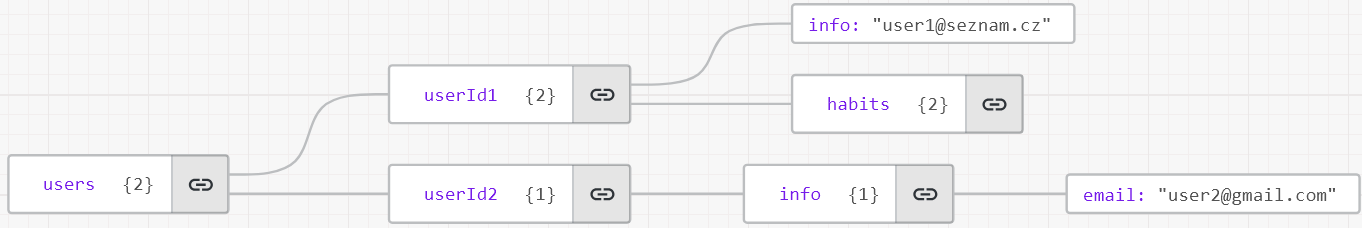
\includegraphics[width=1\linewidth]{images/userschema.png}
    \caption{Users JSON strom}
    \label{fig:users-fb-json}
\end{figure}

\begin{figure}[H]
    \centering
    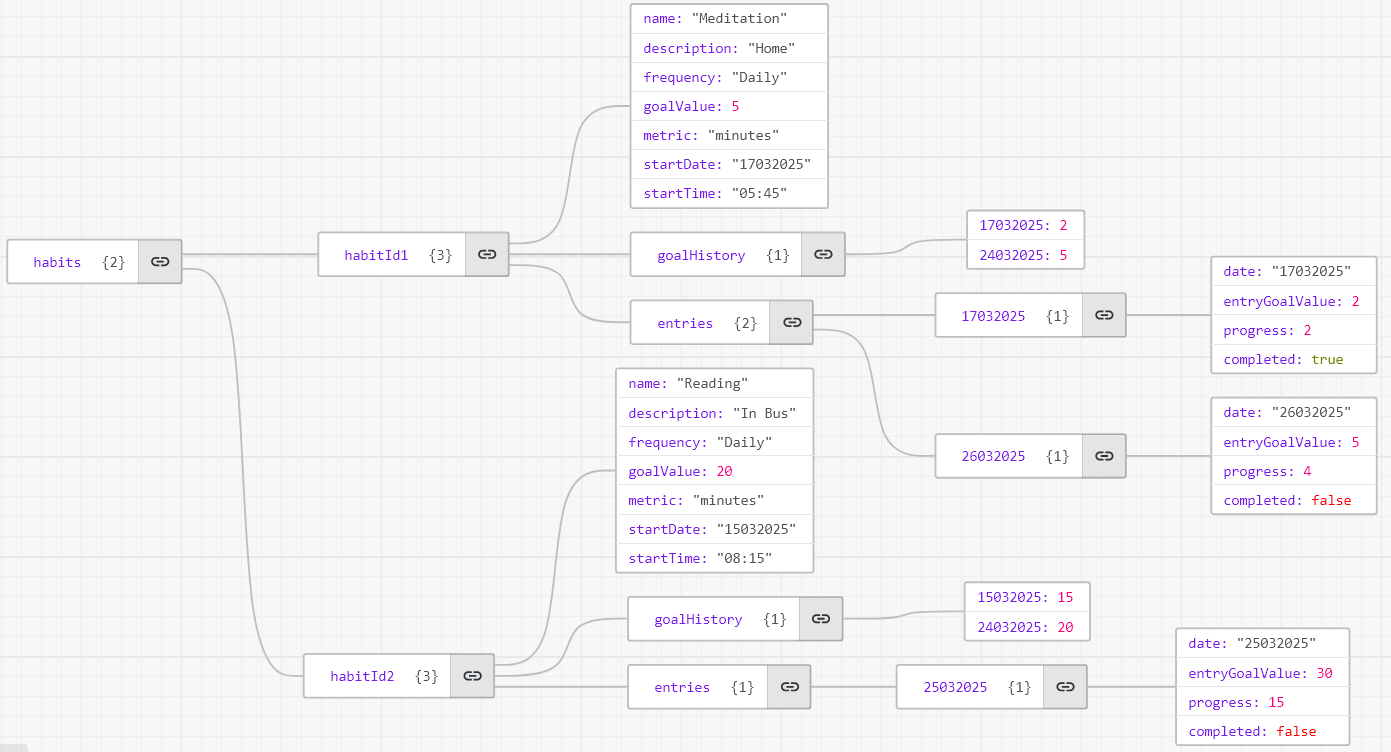
\includegraphics[width=1\linewidth]{images/habitschema.png}
    \caption{Habits JSON strom}
    \label{fig:habits-fb-json}
\end{figure}